\documentclass[a4paper, amsfonts, amssymb, amsmath, reprint, showkeys, nofootinbib, twoside]{revtex4-1}
\usepackage[english]{babel}
\usepackage[utf8]{inputenc}
\usepackage[colorinlistoftodos, color=green!40, prependcaption]{todonotes}
%\input{preamble}
\usepackage[pdftex, pdftitle={Article}, pdfauthor={Author}]{hyperref} % For hyperlinks in the PDF
\usepackage{siunitx}
\newcommand\editremark[1]{{\color{red}#1}}
%\setlength{\marginparwidth}{2.5cm}
%\usepackage{biblatex}
%\addbibresource{Reference.bib}
\bibliographystyle{apsrev4-1}
\begin{document}
\title{Simulating gravitational wave based measurements of the Hubble constant}

\author{noble-alligators}
    %\email[Correspondence email address: ]{email@institution.com}% Your name
    \affiliation{Physics Department, University  of Rochester.}

\date{\today} % Leave empty to omit a date

\begin{abstract}
  In this paper we consider a method for estimating the Hubble constant based on ``dark sirens'', gravitational wave observations which do not have a known electromagnetic counterpart. This method has already been applied to the event GW170814, but more observations are needed to constrain $H_0$ sufficiently to resolve the discrepancy between estimates produced by the Planck collaboration and Riess et al. Using simulated events based on existing gravitational wave detections, we are able to estimate that we will need $90$ observations of black hole mergers  to measure $H_0$ with an uncertainty of $5$ \si{km.s^{-1}.Mpc^{-1}}.
\end{abstract}

\keywords{Hubble's constant, gravitational wave, dark siren}

\maketitle

\section{\label{sec:intro} Introduction}

Hubble's law, the observation that galaxies are moving away from the Earth at a velocity proportional to their distance from the Earth, has been widely accepted since it was first proposed in the 1920s \cite{Hubble_1929}.
The constant of proportionality in this relationship is known as the Hubble parameter $H$.
The Hubble parameter in general changes with time, and therefore with redshift $z$; the current value of the Hubble parameter is the Hubble constant $H_0$.
For objects relatively close to the Earth (i.e. those at low redshift), the redshift is related to the distance $d$ by \cite{Freedman_2010}
\[
    c z = H_0 d.
\]

Variations in the physical assumptions underlying calculations of the Hubble constant, namely those used to compute the distances to objects at particular redshifts, have resulted in differing Hubble constant estimations.
Hubble’s initial estimation, determined by a simple linear fit between recession velocity and distance, gave roughly $500$ \si{km.s^{-1}.Mpc^{-1}} \cite{Hubble_1929}.
Subsequent measurements have progressively refined this estimate, eventually stabilizing at approximately $70$ \si{km.s^{-1}.Mpc^{-1}} \cite{Freedman_2010}.
However, different measurement approaches have led to significant disagreement between estimates: measurement uncertainties continue to diminish as methods improve, but the range of measured values does not.
Figure \ref{fig:hist_h0} gives an overview of recent measurements, showing significant disagreement.

\begin{figure}
    \centering
    \includegraphics[scale=0.7]{H0whisker.pdf}
    \caption{A selection of recent $H_0$ measurements demonstrating the significant discrepancies in its value \cite{Pogosian_2020, Planck_2020, Aiola_2020, WMAP_2018, Henning_2018, Planck_2016, Hinshaw_2013, Freedman_2001, Freedman_2012, Riess_2016, Feeney_2018, Burns_2018,  Riess_2019, Camarena_2020, Riess_2021, Breuval_2021}.}
    \label{fig:hist_h0}
\end{figure}

There are two dominant methods for estimating the Hubble constant which are in tension with one another.
The first uses low redshift measurements of standard candles e.g. type Ia Supernovae, in order to determine $H_0$.
The current estimate using this method is $H_0 = 74.03 \pm 1.42$ \si{km.s^{-1}.Mpc^{-1}} \cite{Riess_2019}.
Another approach, utilizing high redshift measurements of the cosmic microwave background (CMB), gives a value of $H_0 = 67.36 \pm 0.56$ \si{km.s^{-1}.Mpc^{-1}} \cite{Planck_2020}.

It is highly unlikely that the discrepancy between these measurements, at greater than $4\sigma$, can be explained as a statistical fluctuation or through systematic uncertainties.
For instance, Tamara et al. state that even small systematic errors in redshift will have a significant impact on measurements of $H_0$; however, this is not enough to account for the tension in $H_0$ \cite{Davis_2019}.
See e.g. \cite{Efstathiou_2021,Calabrese_2008} for further discussion of systematic uncertainties.

A method for determining $H_0$ that does not rely on standard candles could potentially help resolve the tension in measurements of the Hubble constant.
In this paper we consider an approach utilizing gravitational waves as an independent distance measurement.

%\paragraph{Low redshift ($z \leq 10$) measurement}

%The $H_0$ is calculated locally by measuring the redshift of distant galaxies and then using a particular method to calculate their distances which is part of the cosmic distance ladder.
%The redshift can be easily measured, and the distances can be measured locally by getting the distance from the standard candle techniques, including the Type Ia Supernovae and Cepheid variables.
% \footnote{Astronomers use a “standard candle” to measure distances that are too vast to be measured using parallax. Because the light is spread out over a larger region, distant light sources appear fainter.}

%Tamara et. al gives a statement that even small systematic errors in redshift will result in a significant impact on $H_0$ measurements (2019)\cite{Davis_2019}; however, only considering those errors are not quite enough to resolve the $H_0$ tension people encountered. The research calculation results remain stable with constantly decreasing the error bar, as shown in the figure, except for the results obtained by Freedman et. al. in 2019 shows the relatively low $H_0$ value falls in $69.8 \pm 1.88$ \si{km.s^{-1}.Mpc^{-1}}\cite{Freedman_2019}. Instead of using Cepheid variables, they use the calibration of Tip of the Red Giant Branch(TRGB), which is parallel to but independent from the former one. TRGB samples have higher mass and less sensitivity to the metallicity, so that the potential systematic error in measurement has decreased.

%\paragraph{High redshift ($z \geq 10$) measurement}

%$H_0$ can be calculated using CMB temperature changes. Several characteristics, like the ratio of baryonic to dark matter and $H_0$, influence the specific shape of the curve (known as the acoustic power spectrum). The angular diameter distance to the last scattering surface is used to calculate $H_0$. That isn’t a direct observable; instead, trigonometry is used to infer it. The angular scale of the Baryon Acoustic Oscillations in the CMB may be directly measured, it’s the distance between troughs in the power spectrum is shown below.

%The temperature power spectrum is what is being used to determine the $H_0$. This is a way of looking at the ripples in the temperature field which encode the amount of dark and baryonic matter present, as well as the cosmological constant and other cosmological parameters.
%\footnote{All the parameters are simultaneously constrained with respect to each other using MCMC or other "fitting" approaches. }

%There are two possible systematic errors that are commonly seen. When we use two different likelihood pipelines for the data at certain multipoles, with different parameters used for the calibration efficiencies, it has little effect in reducing the Hubble tension \cite{Efstathiou_2021}. Therefore, the choice of likelihood will result in systematic errors. 
%The second is the systematic error that can occur in the lensing parameter\cite{Calabrese_2008}. The lensing parameter simply rescales by hand the effects of gravitational lensing on the CMB angular power spectra and can be measured by the smoothing of the peaks in the damping tail. This lensing anomaly is not seen in the
%Planck trispectrum data \footnote{CMB lensing} that offer a complementary and independent measurement. If there is no new physics in it, the alternative explanation could be due to a small but still undetected systematic error in the Planck data which can be used to reduce the Hubble Tension.

\section{\label{sec:methods} Methods}

In this paper we consider dark siren measurements, i.e. those which do not have an electromagnetic counterpart.
This is the case for detections of binary black hole hole mergers, which are not expected to have observable EM counterparts.
Though the detection of an EM counterpart can facilitate a determination of host galaxy and therefore result in a well-constrained measurement of $H_0$ \cite{GW170817_H0}, such detections are rare: at time of writing, GW170817 is the only neutron start merger detection with an identified EM counterpart \cite{GW170817_announce}.

As early as 1986 it was proposed that an array of multiple gravitational wave detectors could be used to estimate the distance to an event $d_L$ and bounds on sky location \cite{Schutz_1986}.
These estimates can then be used to produce a catalog of candidate host galaxies from existing sky surveys.
Based on the posterior distributions for these localizations, we use a method for measuring $H_0$ layed out by Nair et al. \cite{Nair_2018}.
It has been predicted that these methods can confine the Hubble constant within the decade \cite{Chen_2018}.
This technique was applied to the event GW170814 by collaborators from the LIGO and Virgo teams using results from the Dark Energy Survey of the southern sky \cite{GW170814_DES}.
We carry out a similar analysis on simulated data sets based on historic GW data and simple physical assumptions for the distribution of galaxies within clusters.

  %I believe leaving the sections in separate files is more organized, change it if you desire 
\section{\label{sec:methods} Methods}


Binary black hole mergers are often called ``dark sirens'' due to their lack observable EM counterparts.
Though the detection of an EM counterpart can facilitate the determination of host galaxy and therefore result in a well-constrained measurement of $H_0$ \cite{GW170817_H0}, such detections are rare: at time of writing, GW170817 is the only neutron start merger detection with an identified EM counterpart \cite{GW170817_announce}.

As early as 1986 it was proposed that an array of multiple gravitational wave detectors could be used to estimate the distance to an event $d_L$ and bounds on sky location \cite{Schutz_1986}.
Gravitational waves originating from a binary black hole system during the inspiral phase of the merger can be used as dark sirens due to the fact that the individual black hole masses can be determined from the gravitational wave frequency.
The power radiating from the binary system is due to its orbital energy, and therefore the power radiating from the source can be determined purely from the gravitational wave frequency, without any knowledge of the luminosity distance.
The power detected is related to this emitted power through an inverse square law, and so the luminosity distance can be determined without the need for a cosmic distance ladder.
Gravitational waves therefore present a completely independent method by which we can determine distances to galaxies, provided we can determine the host galaxy for a given merger \cite{GW170814_DES,GW170817_H0,Nair_2018}.

Since we can estimate the sky location from which the signal was emitted along with the distance to the event, these estimates can then be used to produce a catalog of candidate host galaxies from existing sky surveys.
Based on the posterior distributions for these localizations, we use a method for measuring $H_0$ layed out by Nair et al. \cite{Nair_2018}.
It has been predicted that these methods can confine the Hubble constant within the decade \cite{Chen_2018}.
This technique was applied to the event GW170814 by collaborators from the LIGO and Virgo teams using results from the Dark Energy Survey of the southern sky \cite{GW170814_DES}.
We carry out a similar analysis on simulated data sets based on historic GW data and simple physical assumptions for the distribution of galaxies within clusters.

%\section{Data} \label{sec:develop}

Historic data is taken from merger catalogs from the second and third year of LIGO observations \cite{GWTC_2,GWTC_3}. Our analysis is only interested in the solid angle covered by sky localization ($\Omega$), distances obtained from the GW data ($d_L$), and their uncertainties, $\sigma_d$. We thus marginalize over all other parameters to obtain a three dimensional probability distribution containing only these parameters of interest. It vastly simplifies our analysis if we assume that the uncertainties on $d_L$ are Gaussian. However, posterior distributions from the LIGO papers contain differing upper and lower credible limits. We take the half width on these posteriors as our Gaussian uncertainties.

After obtaining these marginalized probability distributions, we use historic data as a training set for Gaussian kernel density estimation. We then use the kernel estimation to sample simulated events which have the same underlying probability distribution as observations. The returned samples have a finite probability to be from unphysical regions, i.e. $d_L \leq 0$, $\Omega\leq 0$ or $\sigma_d > d_L$. To counteract this, we reject all samples which are outside of the extremal historic values or violate the $\sigma_d \leq d_L$ constraint. Many of the sampled events will have very large localization regions, which makes it inconvenient to use them for estimates of $H_0$. Since our goal is to produce an estimate of how many observations are required to produce estimates of $H_0$ we only perform further analysis on events that were well localized.

After producing simulated GW events we need to select a suitable sky catalog. These data are also simulated by randomly sampling a number of galaxy clusters which are assumed not to interact with one another. The total mass of the cluster is assumed to follow a Press-Schechter mass distribution\cite{Press_1974}. Peculiar motions (which affect the measured redshift $z$) and distance from the center of mass are sampled such that the Virial theorem is obeyed, but other important factors like the very high concentrations of dark matter within clusters are neglected. More details on cluster generation are given in appendix \ref{sec:clust_gen}.
    
%\subsection{\label{Method} Methodology}

We start with a simple application of Bayes' theorem,
\begin{align}
    p(H_0|d_{GW}, d_C)&\propto p(d_{GW}, d_C|H_0)p(H_0)\nonumber\\
    &= p(d_{GW}|H_0)p(d_C|H_0)p(H_0).
\label{eq:bayes}
\end{align}
where $d_{GW}$ refers to the observed data from the gravitational wave detectors and $d_C$ refers to data from the known catalog of stars and their redshifts. We break this joint likelihood into a product of likelihoods since both experiments are statistically independent.

Since we are considering dark sirens without electromagnetic counterparts, we do not know the host galaxy in which the merger occurred. Thus we must marginalize over all possible galaxies within the volume of possible locations supplied by the GW data. Since the number of galaxies is discrete, this is expressed as a sum:

\begin{align}
    p(&d_{GW}, d_C|{z_j, \hat{\Omega}_j},H_0)  \propto  \nonumber\\
    &\sum_{i} w_i \int dV p(d_{GW}|d_L, \hat{\Omega}_{GW}) 
    p(d_C|{z_, \hat{\Omega}_j}) \nonumber\\
    & \delta_D (d_L - d_L(z_i, H_0)) \delta_D (\hat{\Omega}_{GW} - \hat{\Omega}_i).
    \label{eq:marginal_like}
\end{align}
In principle, we should apply a weight to each galaxy $w_i$ we include this in the expression below, but for simplicity we take $w_i=1$ for all galaxies within the volume of interest and $w_i=0$ for all galaxies outside. This same approximation has been used in previous analyses \cite{Chen_2018,GW170814_DES,Nair_2018}. To evaluate this integral we switch to spherical coordinates and work in redshift space as opposed to distance space. This results in a change of coordinates

\begin{equation}
dV \propto \frac{d^2 V}{d z_i d\hat{\Omega}_i} \frac{d z_i}{d r} d r d\hat{\Omega} \propto \frac{r^2(z_i)}{H(z_i)}
\end{equation}
where $H(z_i)$ is the Hubble parameter in redshift space,

\begin{equation}
H(z_i) = H_0^3 \left(\Omega_m (1+z)^3 + \Omega_\Lambda\right)
\end{equation}
where we have assumed a flat universe so $\Omega_k = 0$. We will take $\Omega_m = 0.3$ and $\Omega_\Lambda = 0.7$ in keeping with Soares-Santos et al \cite{GW170814_DES}. We expect our catalog of galaxies to have very low uncertainty on sky location, so we take $p(d_C|z_i,\Omega)=p(d_C|z_i)\delta(\Omega - \Omega_i)$. Finally we can write the posterior distribution for $H_0$:

\begin{align}
     p&(H_0|d_{GW}, d_C)\propto p(H_0) \sum_i \frac{1}{Z_i} \nonumber\\
     &\times \int dz_i p\left(d_{GW}|d_L(z_i, H_0), \hat{\Omega_{i}}\right)p(d_C|z_i)\frac{r^2 (z_i)}{H(z_i)}
    \label{eq: finaleq}
\end{align}
where $d_L(z_i, H_0) = cz_i / H_0$ uses Hubble's law to express luminosity distance in terms of redshift and an assumed value for $H_0$. We assume that the errors on redshifts are Gaussian, in keeping with the analysis by Singer et al. \cite{Singer_2016}. Under this assumption,

\begin{align}
    p&\left(d_{GW}|d_L(z_i, H_0)\right)\propto \nonumber\\
    &\frac{p(\hat{\Omega})}{\sqrt{2\pi}\sigma(\hat{\Omega})} \exp\left(-\frac{(cz_i/H_0 - \hat{d}_{GW})^2}{2\sigma_{GW}^2}\right).
    \label{eq:GW_like}
\end{align}

\section{Results} \label{sec:conclusions}
We produce simulated events until we find at least $100$ with sufficiently small localizations that further analysis is practical.
This cutoff is arbitrary. For all results reported, we used a maximum volume of $0.5\times 10^{9}$\si{Mpc^3}.
We also observed values which had anomalously small localization volumes so we constrained all simulated events to have a localization volume larger than $0.5\times 10^{7}$\si{Mpc^3}.
We found that a total of $650$ observations were needed to produce the desired $100$ well localized events.
These localized regions corresponded to $15.43\%$ of all generated samples.
In all of our tests we injected a known value of $H_0=70$ \si{km.s^{0}.Mpc^{-1}}.

%\begin{figure*}[t]
%    \centering
%    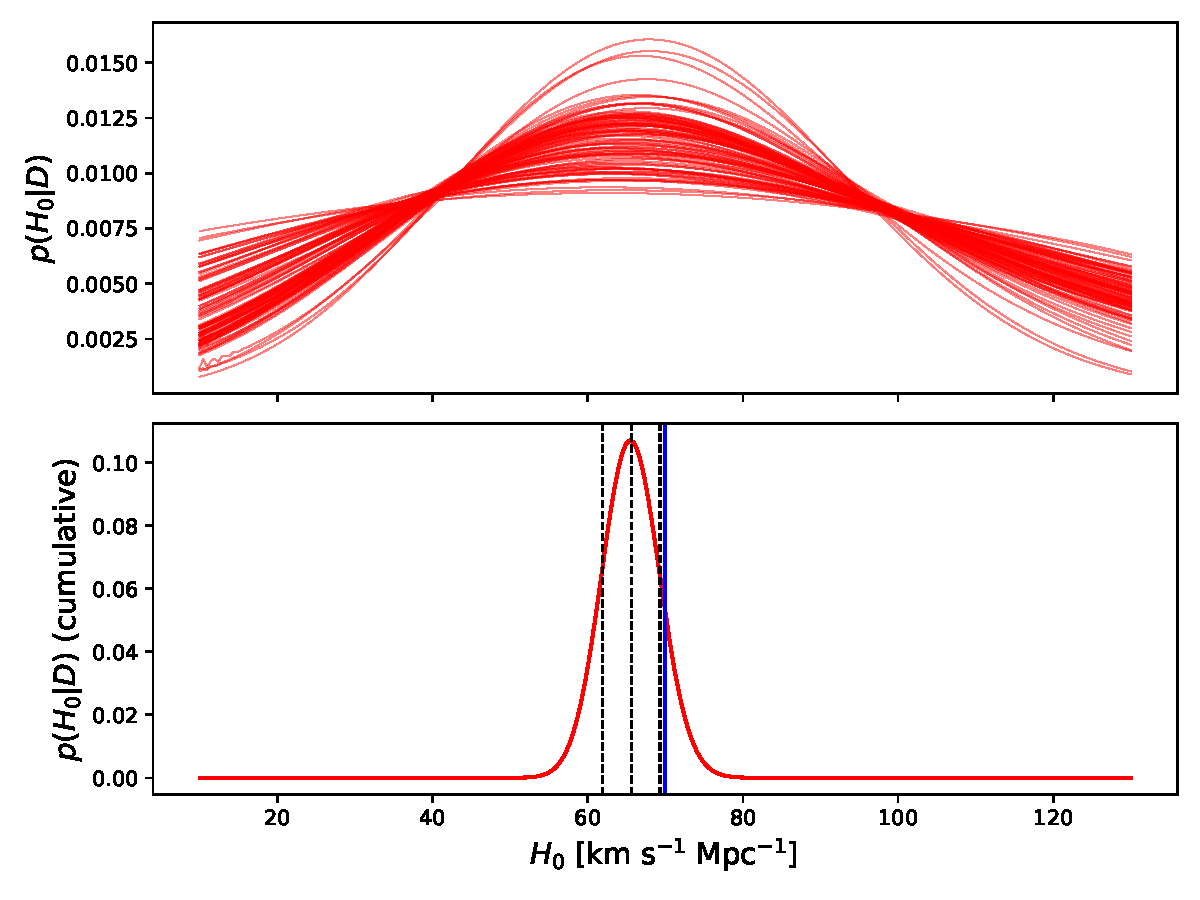
\includegraphics[width=1.5\columnwidth]{figures/posterior.pdf}
%    \caption{Upper: Posteriors produced from individual events. The bias of posteriors with poorer localization is noticable, and is probably contributing to the underestimate of $H_0$ that we note. Lower: The posterior $p(H_0 | d_{GW}, d_C)$ produced after $100$ samples. The $68\%$ credible interval is shown by the dashed lines. The true injected value is shown in blue.}
%    \label{fig:posterior}
%\end{figure*}

\begin{figure}[t]
    \centering
    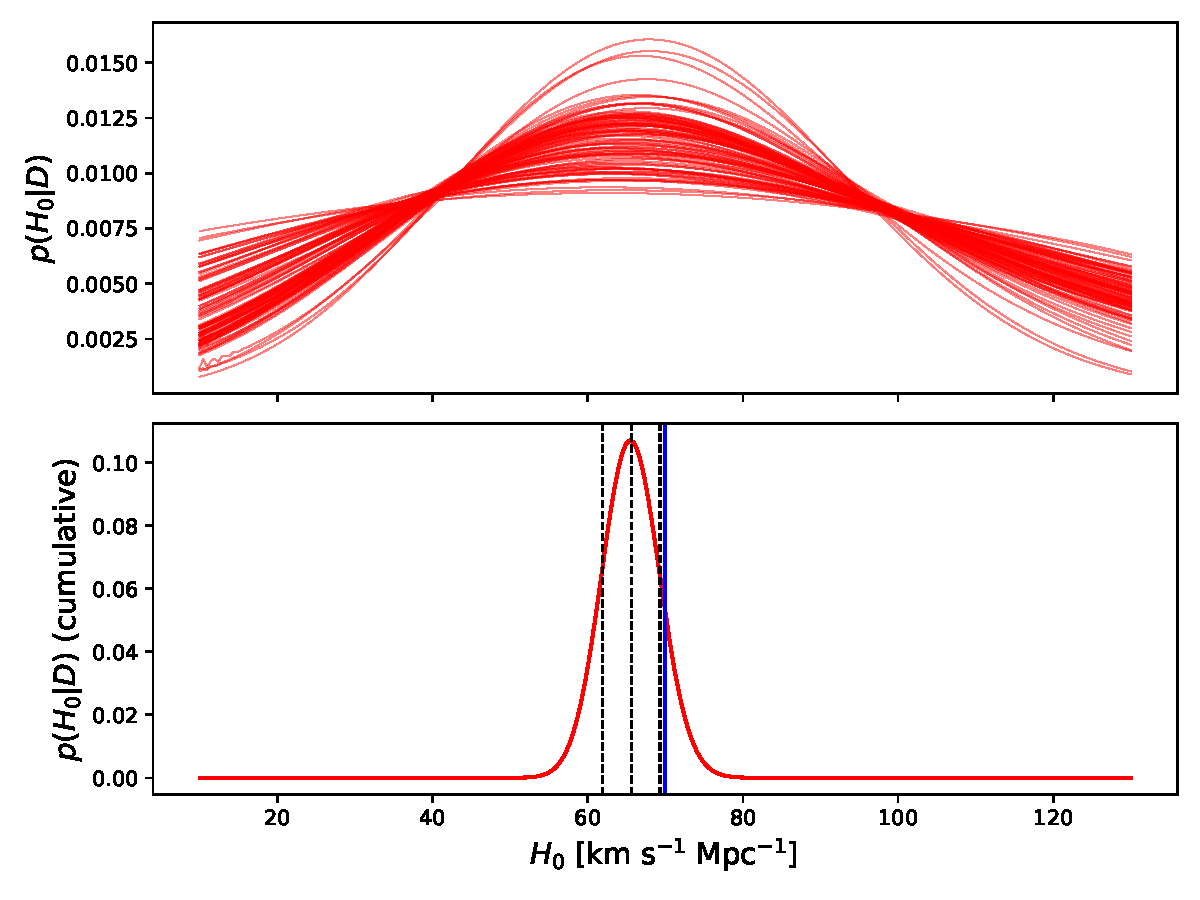
\includegraphics[width=\columnwidth]{figures/posterior.pdf}
    \caption{Upper: Posteriors produced from individual events. The bias of posteriors with poorer localization is noticable, and is probably contributing to the underestimate of $H_0$ that we note. Lower: The posterior $p(H_0 | d_{GW}, d_C)$ produced after $100$ samples. The $68\%$ credible interval is shown by the dashed lines. The true injected value is shown in blue.}
    \label{fig:posterior}
\end{figure}

\begin{figure}
    \centering
    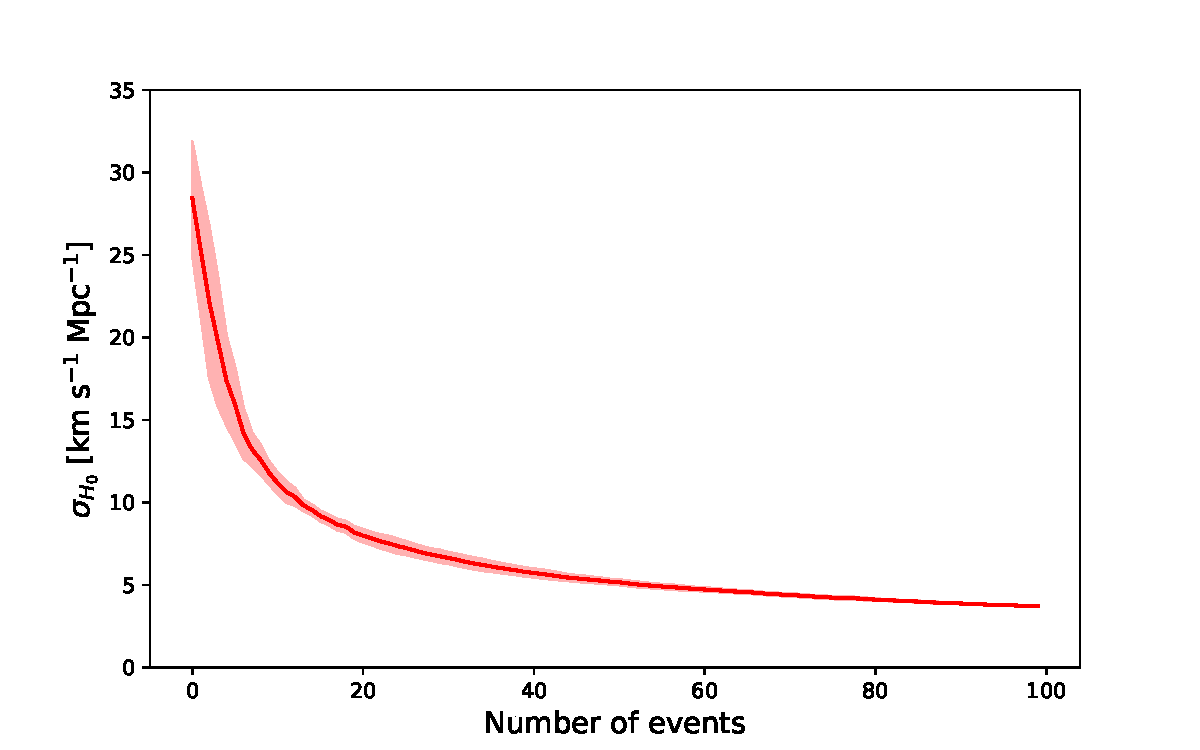
\includegraphics[width=\columnwidth]{figures/std.pdf}
    \caption{The standard deviation obtained from the posterior $p(H_0 | d_{GW}, d_C)$.}
    \label{fig:std}
\end{figure}

\begin{figure}
    \centering
    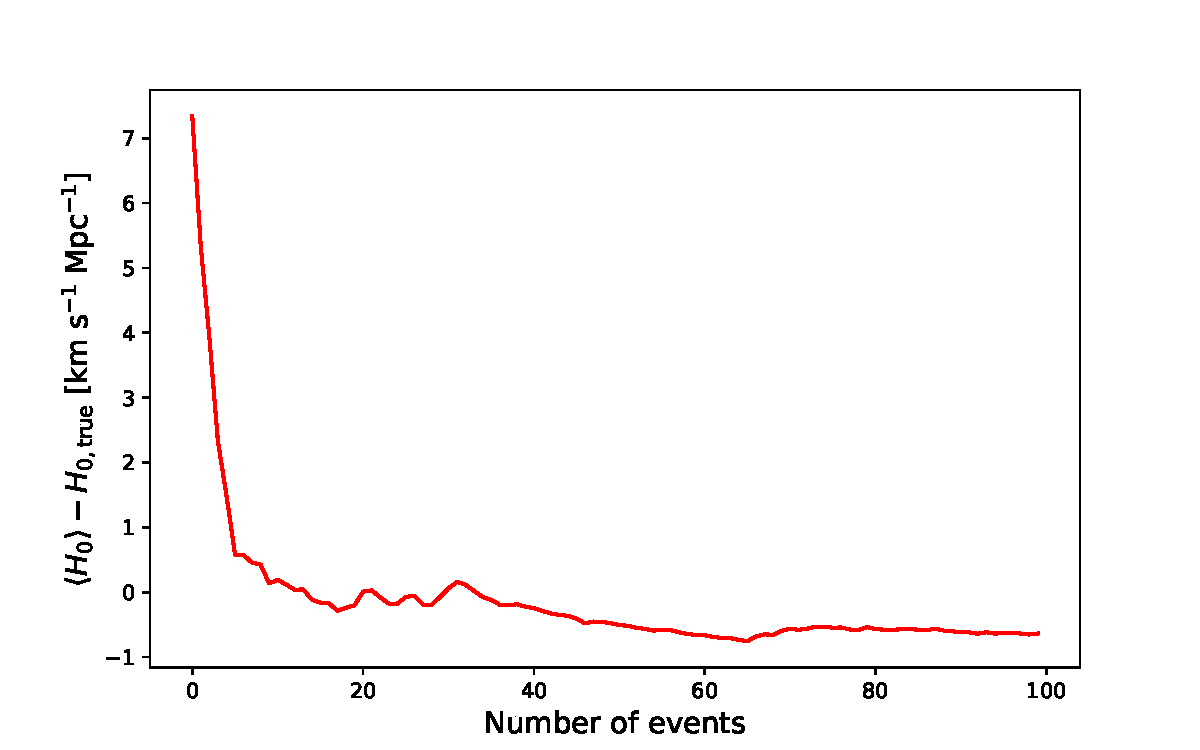
\includegraphics[width=\columnwidth]{figures/diff.pdf}
    \caption{The deviation between the injected known value of $H_0$ and our expectation value based on $p(H_0 | d_{GW}, d_C)$.}
    \label{fig:mean_diff}
\end{figure}

\begin{figure}[t]
    \centering
    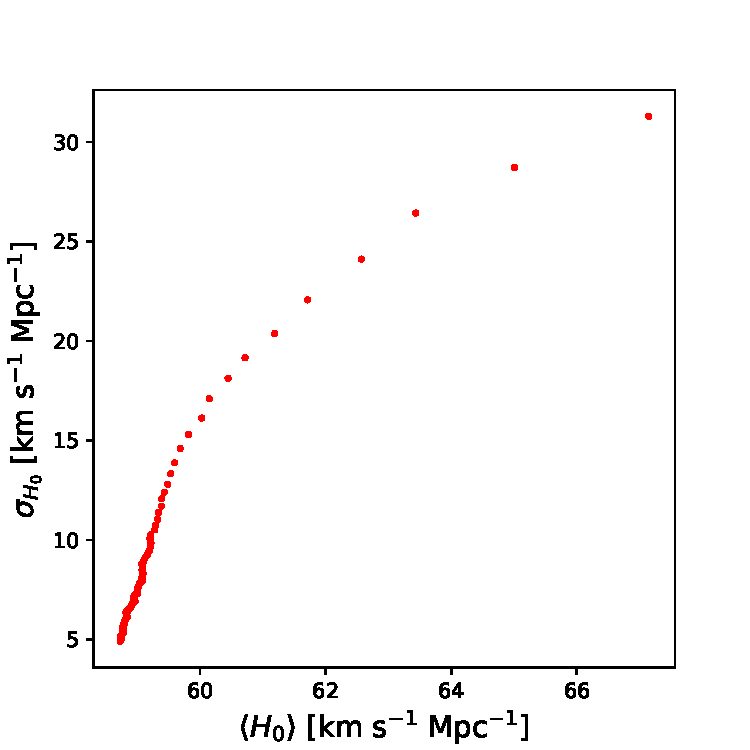
\includegraphics[width=\columnwidth]{figures/correlation.pdf}
    \caption{The means and standard deviations of the estimates on $H_0$ for individual events. Note the clear correlation between these quantities.}
    \label{fig:correlation}
\end{figure}

The resulting posterior $p(H_0 | d_{GW}, d_C)$ produced after $100$ observations is shown in Figure \ref{fig:posterior} along with the posterior obtained from each observation considered in isolation.
In Figure \ref{fig:std} we show the standard deviation of the posterior $p(H_0 | d_{GW}, d_C)$ as a function of number of localized events.
%Some interesting correlations are noticable with events with wider spreads on the posterior tending to center around smaller values of $H_0$.
In Figure \ref{fig:mean_diff} we show the deviation of the posterior expectation on $H_0$ from the known value as a function of number of well localized events.
We can see that our posterior produces an underestimate of $H_0$.
This suggests that there are as yet unidentified systematic effects that need to be taken into account.
Figure \ref{fig:correlation} shows a correlation between the means and standard deviations of the posterior distributions for single events.
This correlation would clearly bias our estimate of $H_0$ towards lower values, since these have smaller standard deviations and thus higher constraining power.
The origin of this correlation is therefore likely to be the unidentified systematic effect.

\section{Discussion} \label{sec:conclusions}

In this paper we have considered a measurement of the Hubble constant $H_0$ using the luminosity distances of binary black hole mergers estimated from their gravitational wave signals.
By simulating the effects of future detections using a physically plausible (though simplified) model of galaxy clusters, we determine that the constraints resulting from such measurements can become considerably smaller.
In particular, we find that after 90 detections with sufficient sky localization, the standard deviation on the measurement of $H_0$ could reach roughly $5$ \si{km.s^{-1}.Mpc^{-1}}.

This measurement of $H_0$ is independent of the standard candles used in other calculations, and thus presents a possible means of confirming or rejecting these other calculations, which are in tension with one another.
However, careful consideration must be given to systematic biases and uncertainties in this analysis.
In particular we see a strong correlation between the measured value of $H_0$ for a particular event and the standard deviation associated with that measurement.
The origin of this correlation is likely to be some systematic bias in the analysis, and future work should determine whether this bias would be present in real data or if it is a result of our simplified galaxy cluster model\footnote{The code for all simulations presented here can be found at: \href{https://github.com/rachel-stromswold/phys403_final_project}{\url{https://github.com/rachel-stromswold/phys403_final_project}}.}.



%\input{sections/acknowledgements.tex}

%\appendix*

%\input{sections/appendix1.tex}

%\bibliography{citations}
%\bibliographystyle{abbrv}
\bibliography{citations}

%\section{GW Event sampling} \label{sec:MCMC}
%To generate simulated gravitational wave data, we first develop an estimate of the probability distribution. This is a very low dimensional probability distribution, with only three variables of interest, luminosity distance, luminosity distance errors and sky location bounds. The training data was taken from the third round of LIGO observations\cite{GWTC_2,GWTC_3}. After the candidate selection is performed, this contains only 76 data points.

%Since this problem is so low dimensional and we have so few data points, we can fairly easily produce a Voronoi tesselation of all observations. The Voronoi tesselation of $N$ is a partition of space with $N$ regions such that each of the $N$ points is contained in exactly one region and all points within the region corresponding to point $i$ are closer to point $i$ than any other point. As such, the reciprocal of the volume of each cell gives an estimate on the density of points within a given region.

%To describe our procedure formally, let $D=\{\vec{x}_i : 1\leq i\leq N\}$ be the set of training points and $\{V_i\}$ be the corresponding set of cells in the Voronoi diagram. Let $NN(\vec{y}):\mathbb{R}^d\to \{i\in\mathbb{N} : 1\leq i\leq N\}$ be the function that maps the point $\vec{y}$ to the index $i$ of its nearest neighbor in the set $D$, and let $v(V_i)$ be the volume of the $i^{th}$ cell. We then assign a probability distribution to each point $\vec{y}\in\mathbb{R}^d$, 

%\begin{equation}
%p(\vec{y} | D) = \left( v( V_{NN(\vec{y})} ) \right)^{-1}
%\end{equation}

%With this probability distribution in place, we can use Markov Chain Monte Carlo to generate event samples.

%It was necessary to rescale the sky location uncertainty by a factor of $1000$ to avoid numeric instabilities before producing tesselations. Training data and MCMC samples are shown in figure \ref{fig:MCMC}

\section{\label{sec:clust_gen} Simulated galaxy catalogs}
After producing a simulated event, we need to produce a catalog of galaxies within the credible interval of sky locations and radial distances obtained from the GW event sample. The volumes produced by typical events are very large, on the order of $1$\si{Gpc^3}. Volumes this lage will exhibit large scale structures. To simplify our analysis we only consider clusters of galaxies and not larger structures such as superclusters or filaments.

To estimate the density of galaxy clusters we use a survey by S. Hansen et al. of a $395$ \si{deg^2} region of sky observed in the SDSS catalog \cite{Hansen_2005}. This analysis found 12830 clusters with redshifts in the range $0.07\leq z\leq 0.3$, for which this catalog is considered complete. Using a value of $H_0=70$ \si{km.s^{-1}.Mpc^{-1}}, we arrive at a very crude estimate of cluster density, $1.5\times 10^{-4}$ \si{Mpc^{-3}}.

Assuming that the mass of normal matter in a cluster follows the Press-Schechter function \cite{Press_1974} and that the number of galaxies is proportional to mass we can express the probability distribution that a cluster has $n$ galaxies,

\begin{equation}
p(n | n_c, \alpha) \propto \left( \frac{n}{n_c} \right)^{\alpha}e^{n/n_c},
\end{equation}
where $n_c$ and $\alpha$ are paramters that should be fitted to the data. Using the same survey mentioned previously we obtain estimates $\alpha = 7.695$ and $n_c = 3$. The authors also find that the characteristic radius for a galaxy cluster goes as $r_c ~ \mathcal{N}_gals^\beta$ for $\beta=0.56$ \cite{Hansen_2005}. We take the offset of any galaxy from the center of mass to follows a three-dimensional Gaussian distribution with $\sigma_r = r_c$. Under the assumption that the virial theorem is obeyed and that velocities follow a normal distribution, we can derive an expression for $\sigma_v$ in terms of $r_c$,

\begin{align}
  \left<U\right> &= \frac{4\pi Gm}{\sqrt{2\pi r_c^2}} \int r e^{-r^2 / 2r_c^2} dr = \sqrt{8\pi m}r_c = 2\pi m\sigma_v^2 = \left<K\right> \nonumber\\
  &\implies \sigma_v^2 = \frac{G r_c}{\sqrt{\pi/2}}.
\end{align}

This model for catalog generation makes a number of unrealistic assumptions. We have treated cluster densities as uniform within the range of interest, but we should expect this to have a redshift dependence. We have also ignored the role of dark matter which should constitute the majority of a cluster's mass. It may be interesting to account for these affects in future work, but the model presented here is sufficient for a toy model. However, this model does produce correlations between the peculiar motions of galaxies and their locations, which is a useful test of the robustness of our estimation of Hubble's constant.

Now that we have described the details of our cluster generation procedure, we need to address one more important detail in our cluster generation. In order to make our data realistic, there should be a true host galaxy. We expect this galaxy to be near the center of our volume credible interval. To account for this, we select a cluster at random to contain the host where the probability that any given cluster contains the host is proportional to the number of galaxies it contains. After selecting this cluster, we move it to the center of the GW localization region and apply a Gaussian displacement.

To get a crude estimate of the width of this Gaussian displacement, we start by considering a sphere which has an equivalent volume. Assuming that this volume represents a $95\%$ confidence interval, the radius of this galaxy should be $2\sigma$. Thus, we select a Gaussian width on the host cluster displacement,

\begin{equation}
  \sigma = \frac{1}{2}\left(\frac{3}{4\pi} V\right)^{1/3}.
\end{equation}

%\section{\label{append_a} Appendix}
%\section{\label{append_b} Appendix}
\end{document}
